\reviewer
% Comment 1
\begin{revcomment}
  The authors should explain the most important achievements of the proposed method quantitatively, in the abstract.
\end{revcomment}
\begin{revresponse}

Thanks for the reviewer's valuable feedback. We have carefully considered this suggestion and made the following modifications to address the reviewer's concern:


By introducing the shortest path($SP$) of the battery, the greedy algorithm transforms the enumeration of switch states in the brute force algorithm into the combination of the $SP$s, which greatly increases the efficiency of determining the maximum allowable current (MAC) of reconfigurable battery systems (RBSs). We have also provided a theoretical estimation of the improved efficiency, which is proportional to $N_s 2^{N_s - N_b} \log_{10} N_b$, where $N_s$ is the number of switches and $N_b$ is the number of batteries.


Here is the specific modification we made in the abstract:
\begin{changes}
  
This paper proposes a method to calculate the MAC of arbitrary RBSs using a greedy algorithm in conjunction with a directed graph model of the RBS.
By introducing the shortest path of the battery, the greedy algorithm transforms the enumeration of switch states in the brute-force algorithm into the combination of the shortest paths, which greatly increases the efficiency with which the MAC is determined.
The directed graph model, based on the equivalent circuit, provides a specific method for calculating the MAC of a given structure.
The proposed method is validated on two published 4-battery-RBSs and one with a more complex structure.
The results are the same as those of the brute-force algorithm, but the proposed method significantly improves the computational efficiency ($N_s 2^{N_s - N_b} \log_{10} N_b$ times faster than the brute force algorithm for a RBS with $N_b$ batteries and $N_s$ switches, theoretically).
The main advantage of the proposed method is its ability to calculate the MAC of RBSs with arbitrary structures, even in scenarios with random isolated batteries.
\end{changes}


We believe that these modifications provide a more quantitative explanation of the achievements of our proposed method in the abstract. 

\end{revresponse}

% Comment 2
\begin{revcomment}
  The literature review in the introduction section is very short, and the related works, especially the works published in recent years, have not been well reviewed and compared, and the conclusions about the existing research gaps have not been presented.
\end{revcomment}
\begin{revresponse}

Considering the Reviewer's suggestion, we have expanded the literature review in the introduction section to provide a comprehensive overview of the existing RBS structures \cite{ci2007novel,9209774,engelhardt2021double,visairoReconfigurableBatteryPack2008,lawsonSoftwareConfigurableBattery2012,he2014reconfiguration,kim2009dynamic} and related works on structure analysis \cite{han2021analysis,chenSneakCircuitTheory2021}. 
Although many RBS structures have been proposed for different purposes, such as dynamically adjusting the output voltage , increasing energy utilization efficiency, and improving the system's ability to recover from battery failures, they also bring challenges in design and control of the systems.
Therefore, several works on structure analysis, like the maximum switch current and the short-circuit problem, have been proposed to tackle these challenges recently.
However, determining the MAC of RBSs remains blank accroding to our literature review.
A straightforward method is to enumerate all possible switch states, but the complexity of this method increases exponentially with the number of switches, and has too ineffection to apply.


Here is the specific modification we made in the introduction:
\begin{changes}
Recently, various types of RBSs with different flexibility and reconfigurability have been designed to meet application requirements. 
For example, Ci et al. \cite{ci2007novel} proposed an RBS structure that dynamically adjusts the battery discharge rate to fully exploit the available capacity of each battery. 
Jan's \cite{9209774,engelhardt2021double} structures  reconfigure structures with variant batteries in series to reach the (constantly changing) voltage requirements during electric vehicle charging.
As shown in Fig. \ref{fig:stru-Visairo}, the structure proposed by Visairo et al. \cite{visairoReconfigurableBatteryPack2008}  changes the system's output voltage based on the load conditions, thereby reducing the power loss of the voltage regulator during the power supply process and improving the efficiency of energy use. 
Also, to enhance the energy efficiency of the system, Lawson et al. \cite{lawsonSoftwareConfigurableBattery2012} and He et al. \cite{he2014reconfiguration}  proposed simplified structures that have fewer switches than Visairo's design.
Kim et al. \cite{kim2009dynamic} improved the system's ability to recover from battery failures by introducing multiple ports into the structure. 


The complex structure between batteries and switches gives RBSs flexibility but also creates challenges in the design and control of the system. 
Thus, several approaches to analyze the RBS structure and performance have been proposed to tackle these challenges.
For instance, 
Han et al. \cite{han2021analysis} derived an analytical expression for the maximum switch current during battery system reconfiguration for a specific RBS structure. 
This helps guide the selection of switches and supports the design of RBS hardware.
Chen et al. \cite{chenSneakCircuitTheory2021} proposed a systematic approach based on  sneak circuit theory to fundamentally avoid the short-circuit problem of RBSs: 
They thoroughly analyzed all paths between the cathode and anode of each battery in the RBS and identified paths that only contain switches as short-circuit paths for pre-checking before system reconfiguration.
\end{changes}

  
Thanks once again for the reviewer's comments, which have greatly improved the quality and comprehensiveness of our manuscript. We believe that the revised introduction section now provides a thorough review of the literature and addresses the existing research gaps in the field of RBS structures.
  
\end{revresponse}

% Comment 3
\begin{revcomment}
  It is necessary for the authors to clearly state research contribution and achievements as bullet points at the end of the Introduction section.
\end{revcomment}
\begin{revresponse}

We appreciate and accept your suggestion and have added a clear statement of the contributions in the second-to-last paragraph of the Introduction, as shown below:
\begin{changes}
The main contributions of this paper can be summarized as follows:
\begin{itemize}
  \item An efficient method is proposed to determine the MAC of RBSs with arbitrary structures, including scenarios with isolated batteries.
  \item The greedy algorithm is applied to solve the MAC problem, the computational complexity of which is greatly reduced compared with the brute-force algorithm.
  \item An improved directed graph model is introduced; it considers the voltage, the internal resistance, the MAC of the battery, and the external load to analyze the current of the RBS.
\end{itemize}
\end{changes}


We believe that these additions enhance the clarity of our manuscript. 

\end{revresponse}

% Comment 4
\begin{revcomment}
  The authors need to present the complexity of their proposed method and compare it with some other state-of-the-art or successful classic methods.
\end{revcomment}
\begin{revresponse}

It is really true as Reviewer suggested about the complexity of our proposed method and the comparison with other state-of-art methods.


We have derived the average time complexity of our proposed greedy algorithm-based MAC determination method to be approximately $O(2^{N_b}N_s^2\log_{10} N_b)$, where $N_b$ and $N_s$ are the number of batteries and switches, respectively.
However, as mentioned in our response to Comment 2, there was a blank in the literature regarding MAC determination methods.
The brute force method, the most straightforward and intuitive method, was used as a benchmark for comparison, whose time complexity is $O(2^{N_s}N_s^3)$.
Since the number of switches in RBS is typically 3 to 5 times the batteries\cite{ciNovelDesignAdaptive2007,alahmadBatterySwitchArray2008,kimDependableEfficientScalable2010b,kimBalancedReconfigurationStorage2011a,taesickimSeriesconnectedSelfreconfigurableMulticell2012a,6843711}, the method we proposed is theoretically more efficient than the brute force method.
It has been validated by the case study in the manuscript.


The detailed derivation and discussion of the above points have been added to the revised manuscript under the Discussion subsection.
Here is the specific modification:
\begin{changes}
The literature contains no report on an algorithm for calculating the MAC of an RBS.
The brute-force algorithm, which goes through all possible switch states, is the most straightforward way to determine the MAC and is used as a benchmark for the proposed greedy algorithm.
If an RBS has $N_b$ batteries and $N_s$ switches and the corresponding directed graph has $N$ nodes,  $2^{N_s}$ iterations are required to traverse all reconfigured structures.
Calculating each reconfigured structure using Eqs. (\ref{eq:I_o})--(\ref{eq:eta}) requires matrix inversion and matrix multiplication, which has a time complexity of $O(N^3+2N^2N_b+N^2N_s+NN^2_b)$.
Therefore, the time complexity of the brute-force algorithm is $O\bm(2^{N_s}(N^3+2N^2N_b+N^2N_s+NN^2_b)\bm)$.
The greedy algorithm proposed in this paper requires  that $SP$ be found for each battery, which requires $N_b$ iterations.
Each $SP$ can be obtained by several applications of Dijkstra's algorithms.
Therefore, the total time complexity for calculating all $SP$s is $O\bm(2N_b(N_b+2N_s)\log_{10} N\bm)$.
According to  Appendix \ref{alg:greedy}, the RBS can reconfigure $C^{N_{\text{set}}}_{N_b}$ structures by selecting $N_{\text{set}}$ batteries from $N_b$ batteries, which gives $\sum^{N_b}_{N_{\text{set}}=1}C^{N_{\text{set}}}_{N_b}/N_b \approx 2^{N_b}/N_b$ on average.
Thus, with the bisection method, the time complexity of the greedy algorithm is $O\bm(2^{N_b}/N_b(N^3+2N^2N_b+N^2N_s+NN^2_b)\log_{10} N_b+2N_b(N_b+2N_s)\log_{10} N\bm)$ [i.e., $O\bm(2^{N_b}/N_b(N^3+2N^2N_b+N^2N_s+NN^2_b)\log_{10} N_b\bm)$].
Based on currently proposed RBS structures \cite{ciNovelDesignAdaptive2007,alahmadBatterySwitchArray2008,kimDependableEfficientScalable2010b,kimBalancedReconfigurationStorage2011a,taesickimSeriesconnectedSelfreconfigurableMulticell2012a,6843711}, the number $N_b$ of batteries, $N_s$ of switches, and $N$ of nodes are quantitatively related as follows: $N_s \approx (3\text{--} 5)N_b$, $N \approx N_s$. 
After simplifying, the time complexity of the greedy algorithm is $O(2^{N_b}N_s^2\log_{10} N_b)$, while it is $O(2^{N_s}N_s^3)$ for brute force algorithm.
Therefore, as the RBS grows, especially in the number of switches, the greedy algorithm gains an advantage over the brute-force algorithm.

This is confirmed by the number of structures required to determine the MAC in the previous section. 
Compared with the brute-force algorithm, the method based on the greedy algorithm is 3\,000 to 48\,000 times more efficient, which is theoretically $N_s 2^{N_s - N_b} \log_{10} N_b$ times according to the above time-complexity analysis.
Of the three RBS structures, the largest is the RBS structure with 19 switches (Fig. \ref{fig:study-stru-my}).
This benefits from two key points:
\begin{enumerate}
\item[(1)] The $SP$s guide the RBS to reconfigure reasonable structures rather than blindly going through all possible structures. This reduces the complexity from $2^{N_s}$ to $2^{N_b}$, which is the main reason for the improvement in efficiency.
\item[(2)] The bisection method further accelerates this process.
\end{enumerate}
\end{changes}

\end{revresponse}

% Comment 5
\begin{revcomment}
  The authors don't discuss the limitations of the study correctly.
\end{revcomment}
\begin{revresponse}

We are sorry for our negligence of the limitations of the study. As far as we are concerned, although the method we proposed is strongly efficient than the brute force method, it still has a exponential relationship with the number of batteries, which means unsufferable time cost will be caused for systems with large number of batteries.


Here is the specific content we added in the discussion:
\begin{changes}
However, the greedy algorithm proposed in this paper still contains exponential terms in the time complexity, which means it may not be able to handle extremely large RBS structures. 
\end{changes}

\end{revresponse}


% Comment 6
\begin{revcomment}
  Some typos should be double check.
\end{revcomment}
\begin{revresponse}

We are very sorry for our incorrect writing, and have carefully checked the manuscript and corrected the typos. 
  
\end{revresponse}

% Comment 7
\begin{revcomment}
  The author should explain more why solution quality of their proposed approach is much better than the others?
\end{revcomment}
\begin{revresponse}

We appreciate the reviewer's concern regarding the explanation of why the solution quality of our proposed approach is better to others. 
However, after careful literature research, we would like to clarify that there are currently no existing works on the MAC determination of RBSs that we could compare our solution with. 
Therefore, it is not possible to directly compare the solution quality of our proposed approach with others.
  
\end{revresponse}

% Comment 8
\begin{revcomment}
  Authors should mention some novel works in the field in the introduction, specially refer to this 2023 reference: An efficient lightweight algorithm for scheduling tasks onto dynamically reconfigurable hardware using graph-oriented simulated annealing, which uses graph-based method. Mention and refer to it in the introduction section.
\end{revcomment}
\begin{revresponse}

Thanks to the reviewer's suggestion, we have introduced two novel works in the RBS structure analysis field in the introduction, which respectively study the maximum switch current \cite{han2021analysis} and the short-circuit problem \cite{chenSneakCircuitTheory2021} in RBS structures.
We believe that these works represent the innovation and recent advances in the field of RBS structure analysis.


The reviewer also specially mentioned the work published in 2023: An efficient lightweight algorithm for scheduling tasks onto dynamically reconfigurable hardware using graph-oriented simulated annealing.
We have carefully read this paper, and after fully discussion, we finally agreed that this paper is not relevant to our research.
Although this paper uses a graph-based method, whose name is similar to the method described in our paper, it mainly studies the task scheduling problem in time series.
While our research is about the maximum allowable current of RBS structure, which belongs to the field of structure analysis.
Therefore, we believe that it is not appropriate to include this paper in our introduction and will not cite it.
  
\end{revresponse}

% Comment 9
\begin{revcomment}
  Authors need to explain about the accuracy, sufficiency and reliability of their results? How do they verify and validate the results?
\end{revcomment}
\begin{revresponse}

TODO: discuss with Qian and Xu

Thanks for the reviewer's valuable feedback. We have carefully considered the reviewer's question.
In response, we complemented the computation with the brute force method and provided more detailed explanation and discussion.


In the Case Study section of the paper, we investigated the MACs of three RBS structures, two of which are from published literatures \cite{lawsonSoftwareConfigurableBattery2012,visairoReconfigurableBatteryPack2008} and the other is designed by ourselves, as shown in Figure \ref{fig:study-stru-Lawson}, \ref{fig:study-stru-Visairo} and \ref{fig:study-stru-my}, respectively.
The results of the three RBS structures calculated by our proposed method are shown in Tables \ref{tab:study-results-Lawson-greedy}, \ref{tab:study-results-Visairo-greedy} and \ref{tab:study-results-my-greedy}, respectively.
The results by brute force method are shown in Tables \ref{tab:study-results-Lawson-brute}, \ref{tab:study-results-Visairo-brute} and \ref{tab:study-results-my-brute}, respectively.


On the one hand, as shown in the Tables \ref{tab:study-results-Lawson-greedy} to \ref{tab:study-results-my-brute}, the reconfigured structure results from our greedy algorithm are consistent with the results from the brute force algorithm, which enumerates all possible reconfigured structures.
It shows that our algorithm does find the global optimal solution.
On the other hand, the output current of the system calculated by our directed graph model is consistent with the experience and common sense.
To illustrate this, the RBS structure shown in Figure \ref{fig:study-stru-my} is taken as an example here.
The four batteries in this structure can be divided into two groups: $B_1$ and $B_2$, $B_3$ and $B_4$.
The relationship between the two batteries in each group can be switched between series and parallel by reconfiguration.
While the two groups can only form a series connection or be disconnected, rather than a parallel connection.
Therefore, the MAC of this structure is the maximum of the output current of the two groups, which is twice the maximum allowable current of a single battery, consistented with the result $\max \eta = 2$ shown in Table \ref{tab:study-results-my-greedy}.


We hope that our above content can address the reviewer's concerns.

% \begin{figure}[htbp]
%     \centering
%     \begin{subfigure}[b]{0.2\textwidth}
%         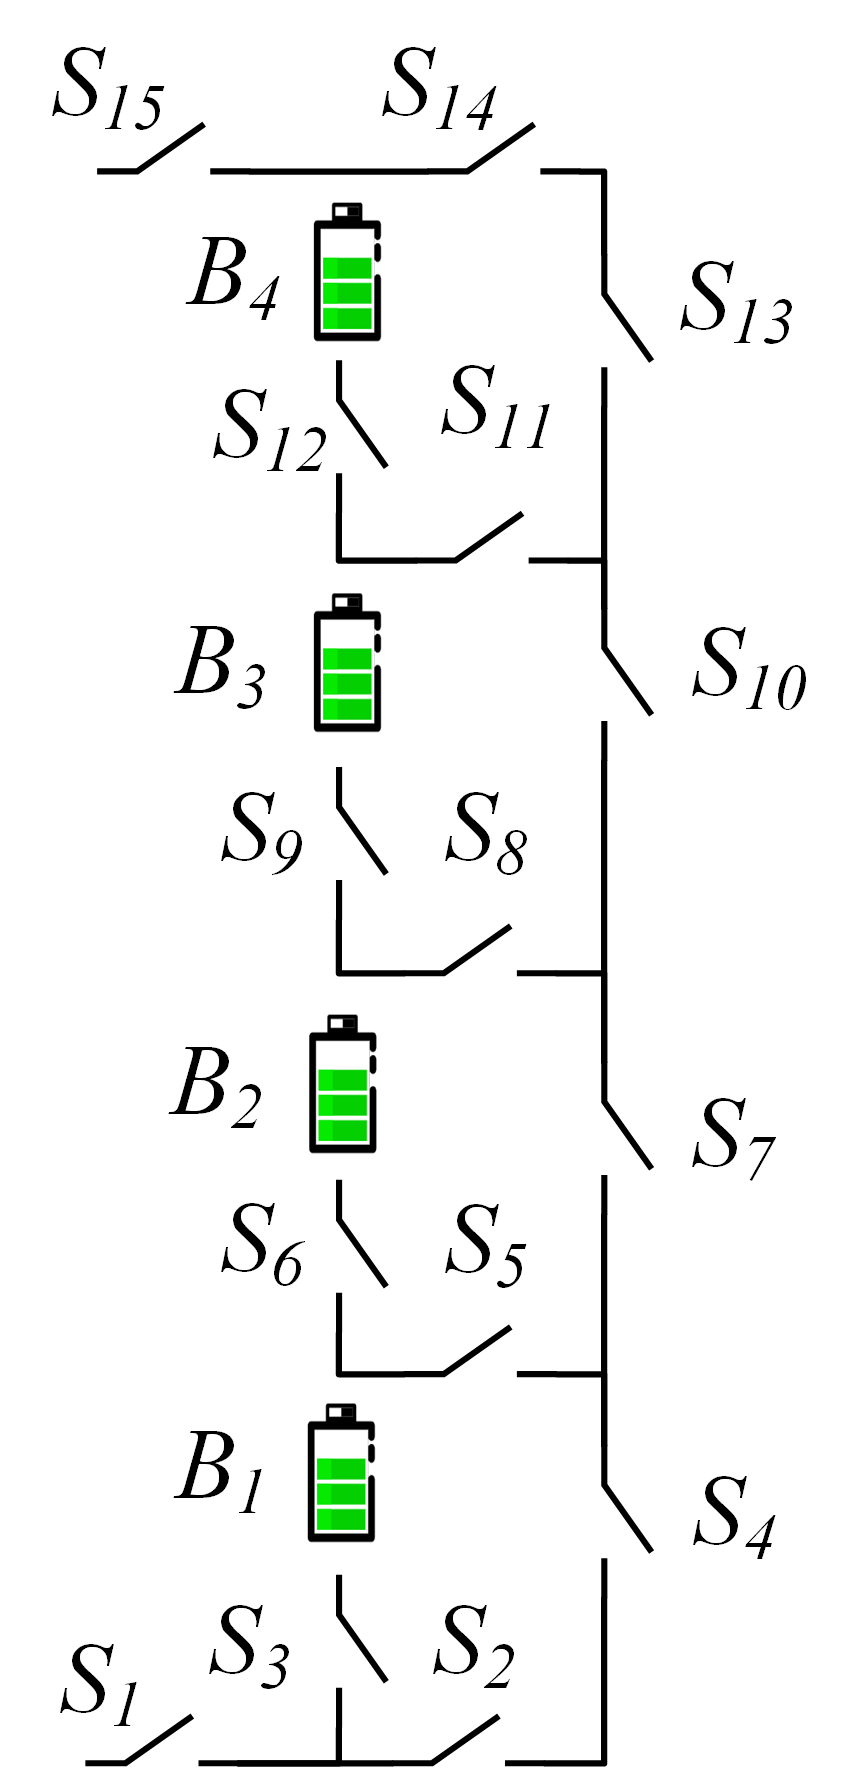
\includegraphics[width=\textwidth]{stru-L-origin.png}
%         \caption{}
%         \label{fig:study-stru-Lawson}
%     \end{subfigure}
%     \hspace{0.02\textwidth}
%     \begin{subfigure}[b]{0.4\textwidth}
%         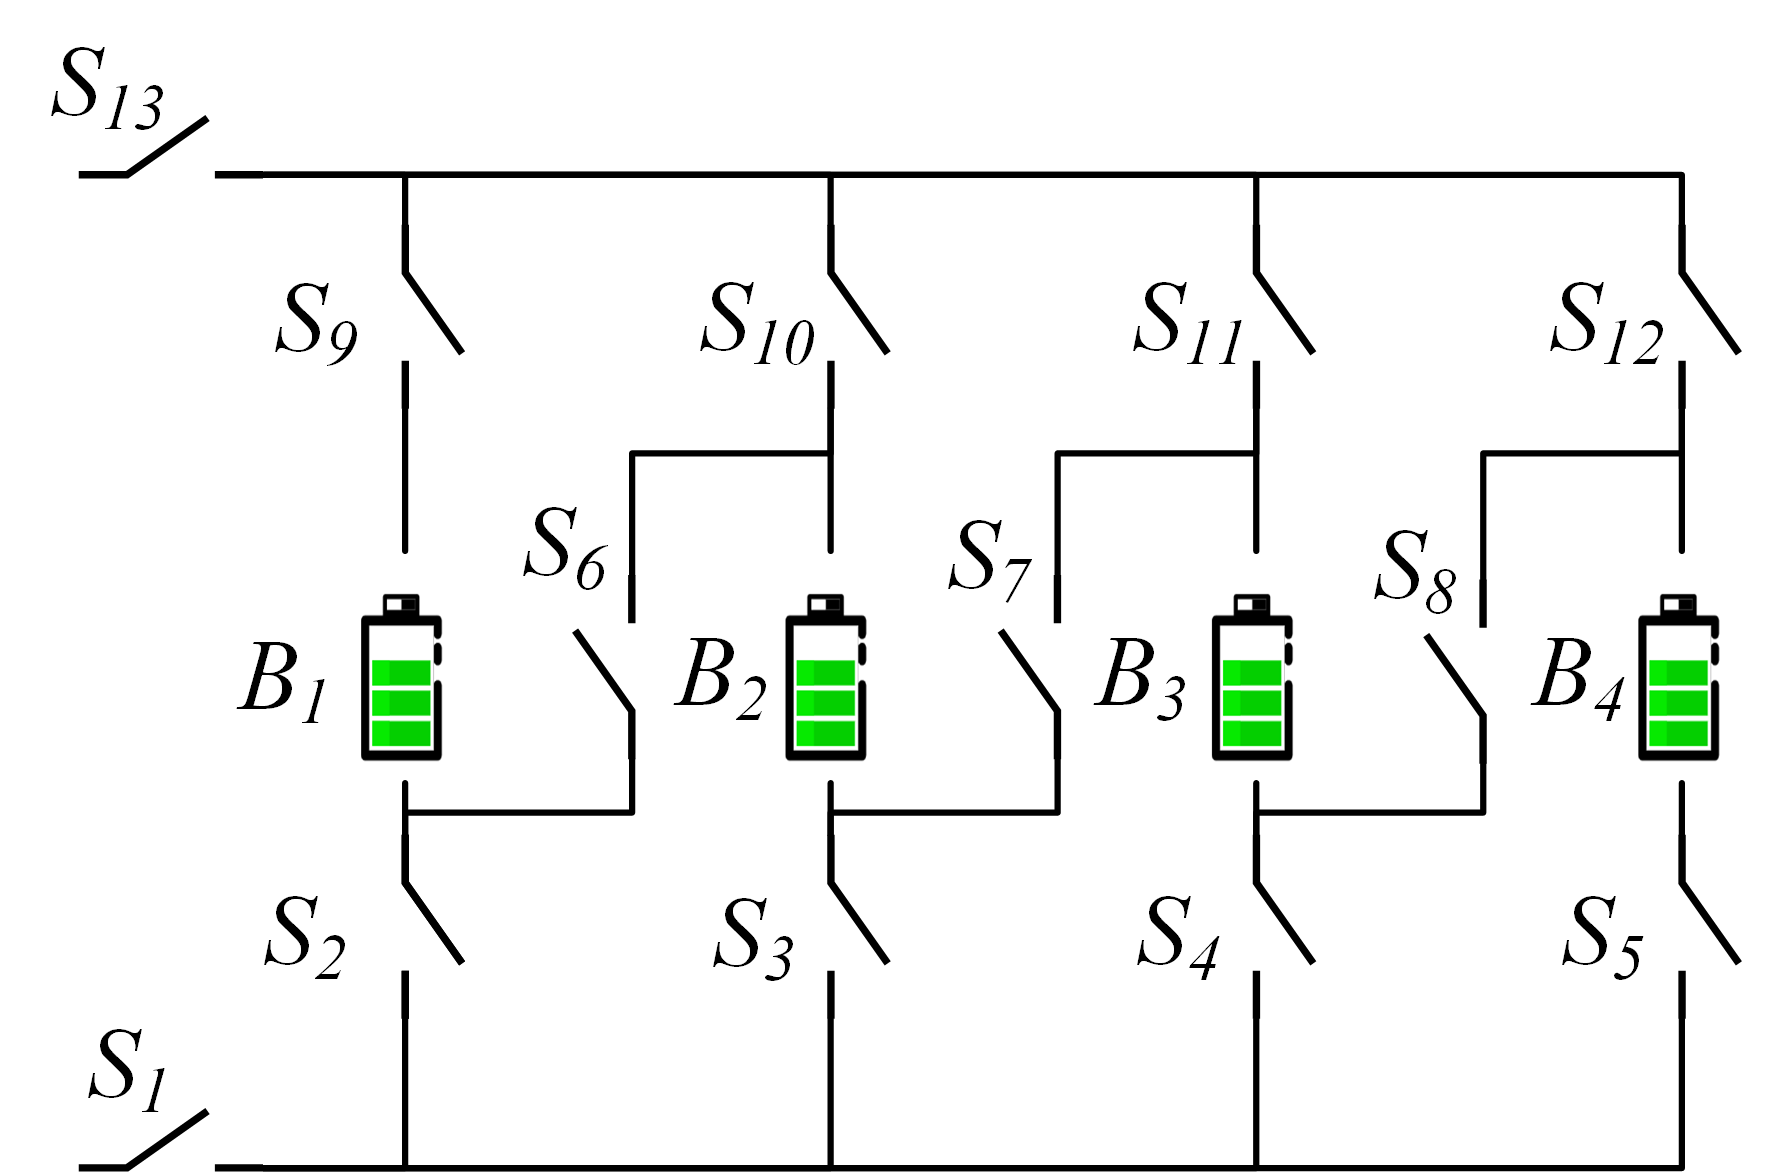
\includegraphics[width=\textwidth]{stru-V-origin.png}
%         \caption{}
%         \label{fig:study-stru-Visairo}
%     \end{subfigure}
%     \hspace{0.02\textwidth}
%     \begin{subfigure}[b]{0.31\textwidth}
%         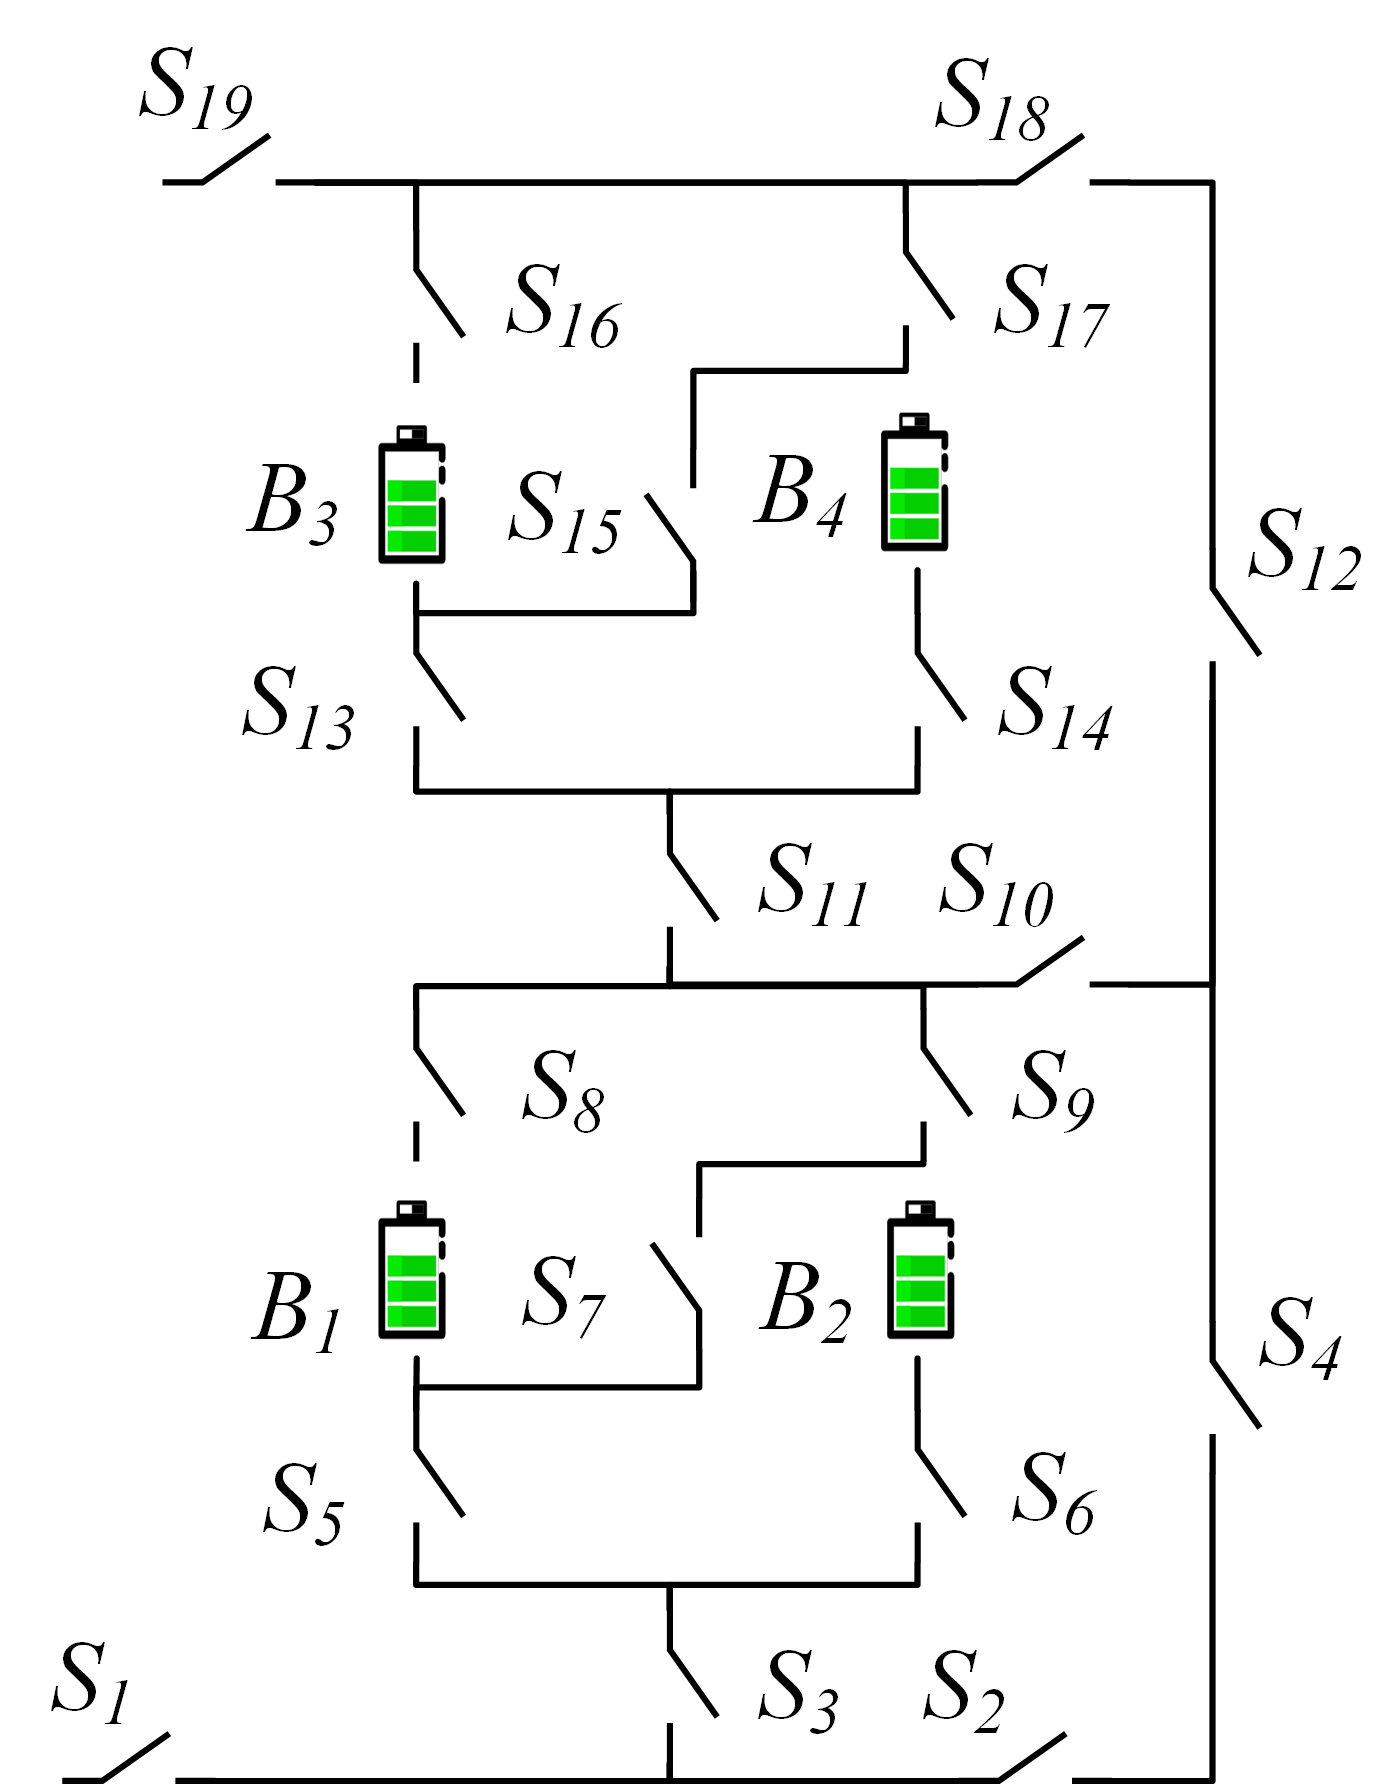
\includegraphics[width=\textwidth]{stru-my-origin.png}
%         \caption{}
%         \label{fig:study-stru-my}
%     \end{subfigure}
%     \caption{The 4-battery RBS structures proposed by (a)Lawson\cite{lawsonSoftwareConfigurableBattery2012}, (b)Visairo\cite{visairoReconfigurableBatteryPack2008} and (c)this paper.}
% \end{figure}

\begin{table}[htbp]
  \centering
    \caption{MAC Calculating result of the RBS structure in Figure \ref{fig:study-stru-Lawson} with our method.}
    \begin{tabular}{cc}
    \toprule
        Structure & Figure \ref{fig:study-stru-Lawson} with 4 batteries and 15 switches  \\
    \midrule
    Switch ON & $S_1$,$S_3$,$S_5$,$S_7$,$S_{10}$,$S_{13}$,$S_{14}$,$S_{15}$ \\
    $I_o$ & $u_b/(R_o+r_b)$ \\
    $\bm{I}_b$ & $[u_b/(R_o+r_b),0,0,0]$ \\
    $\max  \eta$     & 1 \\
    computed structure count & 11 \\
    \bottomrule
    \end{tabular}
  \label{tab:study-results-Lawson-greedy}
\end{table}

\begin{table}[htbp]
  \centering
    \caption{MAC Calculating result of the RBS structure in Figure \ref{fig:study-stru-Visairo} with our method.}
    \begin{tabular}{cc}
    \toprule
        Structure & Figure \ref{fig:study-stru-Visairo} with 4 batteries and 13 switches  \\
    \midrule
    Switch ON & $S_1$,$S_2$,$S_3$,$S_4$,$S_5$,$S_9$,$S_{10}$,$S_{11}$,$S_{12}$,$S_{13}$ \\
    $I_o$ & $4u_b/(4R_o+r_b)$ \\
    $\bm{I}_b$ & $[u_b/(4R_o+r_b),u_b/(4R_o+r_b),u_b/(4R_o+r_b),u_b/(4R_o+r_b)]$ \\
    $\max \eta$     & 4 \\
    computed structure count & 1 \\
    \bottomrule
    \end{tabular}
  \label{tab:study-results-Visairo-greedy}
\end{table}

\begin{table}[htbp]
  \centering
    \caption{MAC Calculating result of the RBS structure in Figure \ref{fig:study-stru-my} with our method.}
    \begin{tabular}{cc}
    \toprule
        Structure & Figure \ref{fig:study-stru-my} with 4 batteries and 19 switches  \\
    \midrule
    Switch ON & $S_1$,$S_3$,$S_5$,$S_6$,$S_8$,$S_9$,$S_{10}$,$S_{12}$,$S_{18}$,$S_{19}$ \\
    $I_o$ & $2u_b/(2R_o+r_b)$ \\
    $\bm{I}_b$ & $[u_b/(2R_o+r_b),u_b/(2R_o+r_b),0,0]$ \\
    $\max  \eta$     & 2 \\
    computed structure count & 11 \\
    \bottomrule
    \end{tabular}
  \label{tab:study-results-my-greedy}
\end{table}

\begin{table}[htbp]
  \centering
    \caption{MAC Calculating result of the RBS structure in Figure \ref{fig:study-stru-Lawson} with brute force method.}
    \begin{tabular}{cc}
    \toprule
        Structure & Figure \ref{fig:study-stru-Lawson} with 4 batteries and 15 switches  \\
    \midrule
    Switch ON & $S_1$,$S_3$,$S_5$,$S_7$,$S_{10}$,$S_{13}$,$S_{14}$,$S_{15}$ \\
    $I_o$ & $u_b/(R_o+r_b)$ \\
    $\bm{I}_b$ & $[u_b/(R_o+r_b),0,0,0]$ \\
    $\max \eta$     & 1 \\
    computed structure count & 32768 \\
    \bottomrule
    \end{tabular}
  \label{tab:study-results-Lawson-brute}
\end{table}

\begin{table}[htbp]
  \centering
    \caption{MAC Calculating result of the RBS structure in Figure \ref{fig:study-stru-Visairo} with brute force method.}
    \begin{tabular}{cc}
    \toprule
        Structure & Figure \ref{fig:study-stru-Visairo} with 4 batteries and 13 switches  \\
    \midrule
    Switch ON & $S_1$,$S_2$,$S_3$,$S_4$,$S_5$,$S_9$,$S_{10}$,$S_{11}$,$S_{12}$,$S_{13}$ \\
    $I_o$ & $4u_b/(4R_o+r_b)$ \\
    $\bm{I}_b$ & $[u_b/(4R_o+r_b),u_b/(4R_o+r_b),u_b/(4R_o+r_b),u_b/(4R_o+r_b)]$ \\
    $\max \eta$     & 4 \\
    computed structure count & 8192 \\
    \bottomrule
    \end{tabular}
  \label{tab:study-results-Visairo-brute}
\end{table}

\begin{table}[htbp]
  \centering
    \caption{MAC Calculating result of the RBS structure in Figure \ref{fig:study-stru-my} with brute force method.}
    \begin{tabular}{cc}
    \toprule
        Structure & Figure \ref{fig:study-stru-my} with 4 batteries and 19 switches  \\
    \midrule
    Switch ON & $S_1$,$S_3$,$S_5$,$S_6$,$S_8$,$S_9$,$S_{10}$,$S_{12}$,$S_{18}$,$S_{19}$ \\
    $I_o$ & $2u_b/(2R_o+r_b)$ \\
    $\bm{I}_b$ & $[u_b/(2R_o+r_b),u_b/(2R_o+r_b),0,0]$ \\
    $\max \eta$     & 2 \\
    computed structure count & 524288 \\
    \bottomrule
    \end{tabular}
  \label{tab:study-results-my-brute}
\end{table}

\end{revresponse}